\subsection{User interface}\label{UI_Design}
The user interface(UI) is a critical part of the audio DSP project. The UI makes it that the user can interact with the system and set his desired settings.
What makes a good UI design is consistency, Readability and feedback. If every menu has the same style and general button layout to make sure menus are easy to navigate. Text in the UI should be kept to a minimum. This follows the saying that an image is worth a thousand words.If text is necessary it should be easy to read. The U should provide proper feedback, this means that if for example a page would take a second to load the UI should show that it is loading a page to prevent frustrations and possible errors.

\subsubsection{UI Components}
The UI will consist of the following three main components: A touchscreen, a rotary knob (with pushbutton) and a controller. The screen is a Nextion screen, meaning the menu design can be done in the Nextion editor.
The benefit of this is that we can design a menu in photoshop and lay transparent buttons on top of the parts that the user should be able to press.

The controller can control the screen visuals by sending commands via UART protocol. When an on screen button is pressed the Nextion screen sends can send the id of the button which is pressed. The menu navigation can be entirely done by using the rotary knob with pushbutton, but the screen also is a touchscreen so for simplicity's sake every on screen button can be used with touchscreen as well.

\subsubsection{UI Design}
The design was started with a diagram with all the necessary screens and information so that is was clear what menus should be in the DSP. There are 2 main menu layouts which are considered, namely function based and channel based. The function based layout is a layout where the functions are grouped and at the lowest level possible the channel has to be selected, for example in the function based layout the user would first navigate to the equalizer section and then select for which channel the equalizer has to be set.

The channel based layout is a layout where the user first selects the main functionality (signal routing, effects or presets) and after that selects the channel giving the user specific controls for the selected channel all in one place. Lets take a look at the previous example in the function based layout. In this case the user would navigate to the effect section, than select the channel to modify and lastly selecting the effect, in this case the equalizer.

\begin{figure}[ht]
    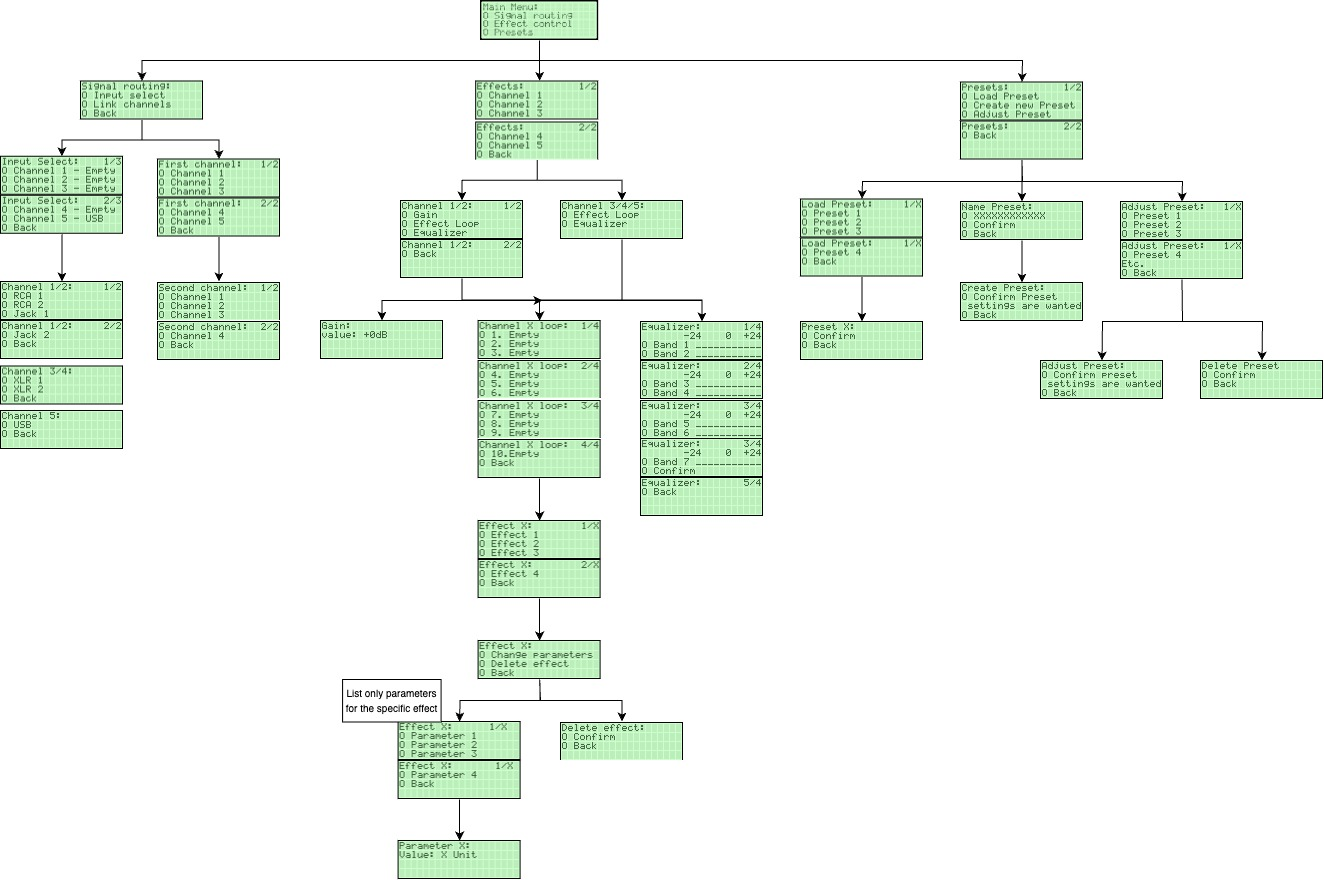
\includegraphics[width=\linewidth]{functionbasedUI}
    \caption{Function Based UI Design for a liquidCrystal screen}
    \label{fig:functionbasedUI}
\end{figure}

The channel based layout is chosen for the audio DSP UI, because it gives the user better overview of settings of the DSP, because all functions are sorted per channel.

\subsubsection{UI controller}
The main component of the UI is the UI controller, it translates commands from the user to commands the signal processer manager can interpret. The block diagram is shown in \ref{fig:UIcontroller-block-diagram}. The UI controller stores every effect parameter, channel routing and preset data in its memory. Whenever an effect parameter changes the Menu controller sends the new data to the signal processor manager, for it to take this new value into account. 

\begin{figure}[ht]
    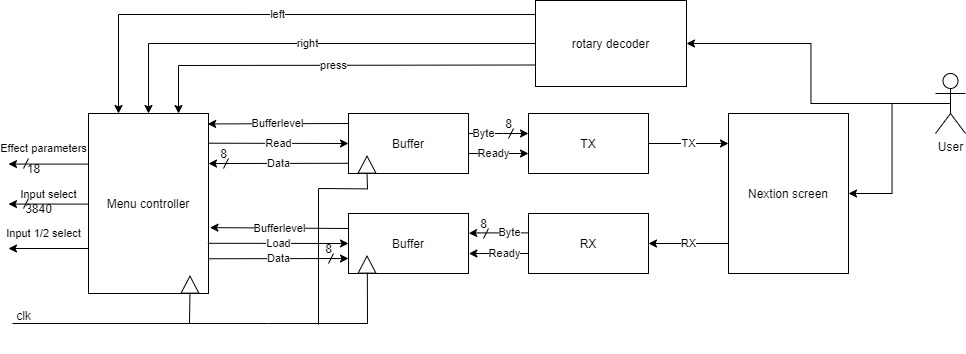
\includegraphics[width=\textwidth]{UI controller block diagram}
    \caption{Overview of UI controller block}
    \label{fig:UIcontroller-block-diagram}
\end{figure}

\paragraph{Menu controller}
The menu controller is the block that contains all the logic for the menu navigation and DSP control. It reads user inputs coming from the touchscreen or from the rotary encoder, and processes that into menu navigation and updating the correct parameters. The controller checks in the RX buffer for the stop bytes and if they are there then it starts processing the incoming data, and perform the appropriate actions.

\paragraph{Buffer}
The buffer block is a circular FIFO buffer, meaning that the data comes in and the buffer keeps track of the position of the first unread byte, called the tail, and the next free space in the buffer, called the head. When a new byte comes in the byte is placed at head. When a byte is read the buffer takes it from the tail. When the head or tail reaches the end of the buffer it cycles back to the beginning of the buffer. In the case that the head and the tail are at the same position the buffer is either completely full or empty.

\paragraph{Tx}
The TX block is capable of sending a single byte at a time. When the ready line is high the block loads the data on the Byte line and sends the bits one by one at the set baud rate.

\paragraph{RX}
The RX block is capable of receiving a single byte at a time. When a full byte has been received the data gets put on the Byte line and the ready line will be high for a single clock cycle.

\paragraph{Memory}
The memory block is a simple register which stores frames of 32 bits at an address. It has 7 bit addresses meaning 128 frames can be stored, which is enough to hold the 120 frames which are necessary to store the 120 effect parameters.

\paragraph{Nextion screen}
The nextion screen used in this project is an 3,5" discovery version screen with 320x480 pixels. The screen has its own controller which is responsible for handling incoming commands, send commands when the screen is touched and most importantly load the menu's to the screen. Figure \ref{fig:mainmenu} shows the home screen of the UI. These screens are designed in Adobe and imported to the Nextion environment with invisible buttons on top of the image.

Figure \ref{fig:adjustpresetmenu} shows what the majority of the menu's look like. The three banner style with the action described in short text.